\documentclass[12pt]{article}
\usepackage{packages}

\begin{document}
\section*{Exercise 1}
\begin{figure}[h]
\begin{minipage}{0.3\textwidth}
    \includegraphics[width=1.2\textwidth]{figures/lib1.eps}
    \caption{Mersenne Twister 19937}
\end{minipage}
\begin{minipage}{0.3\textwidth}
    \includegraphics[width=1.2\textwidth]{figures/builtin1.eps}
    \caption{c++ rand()}
\end{minipage}
\begin{minipage}{0.3\textwidth}
    \includegraphics[width=1.2\textwidth]{figures/randu1.eps}
    \caption{RANDU}
\end{minipage}
\end{figure}
\begin{figure}[h]
    \begin{minipage}{0.3\textwidth}
        \includegraphics[width=1.2\textwidth]{figures/lib.eps}
        \caption{Mersenne Twister 19937}
    \end{minipage}
    \begin{minipage}{0.3\textwidth}
        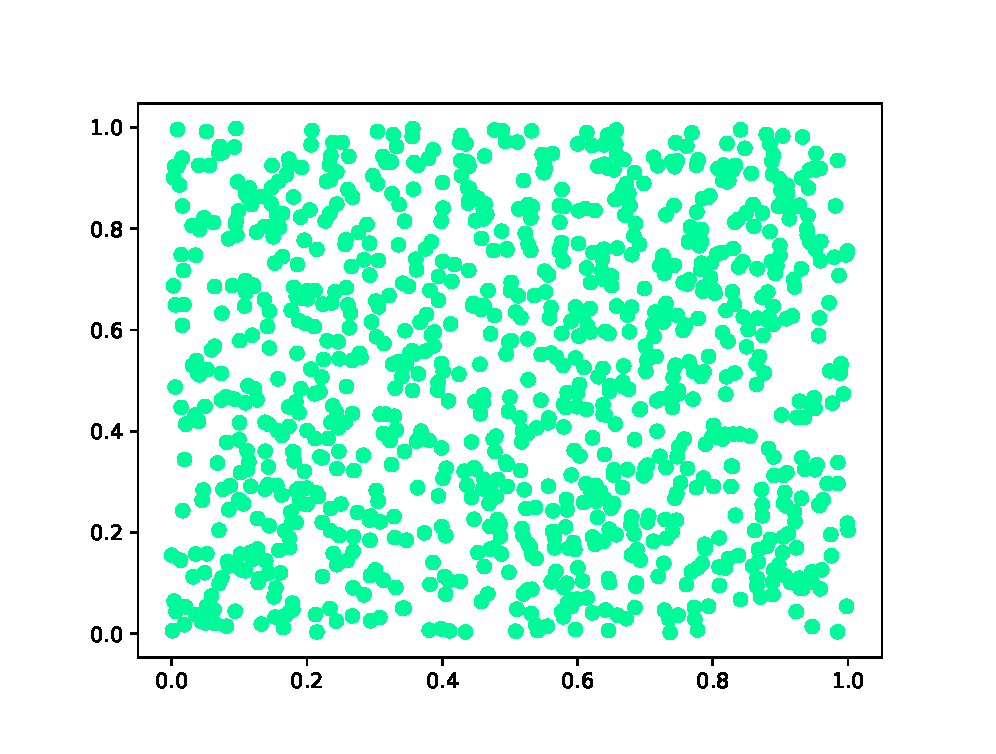
\includegraphics[width=1.2\textwidth]{figures/builtin.eps}
        \caption{c++ rand()}
    \end{minipage}
    \begin{minipage}{0.3\textwidth}
        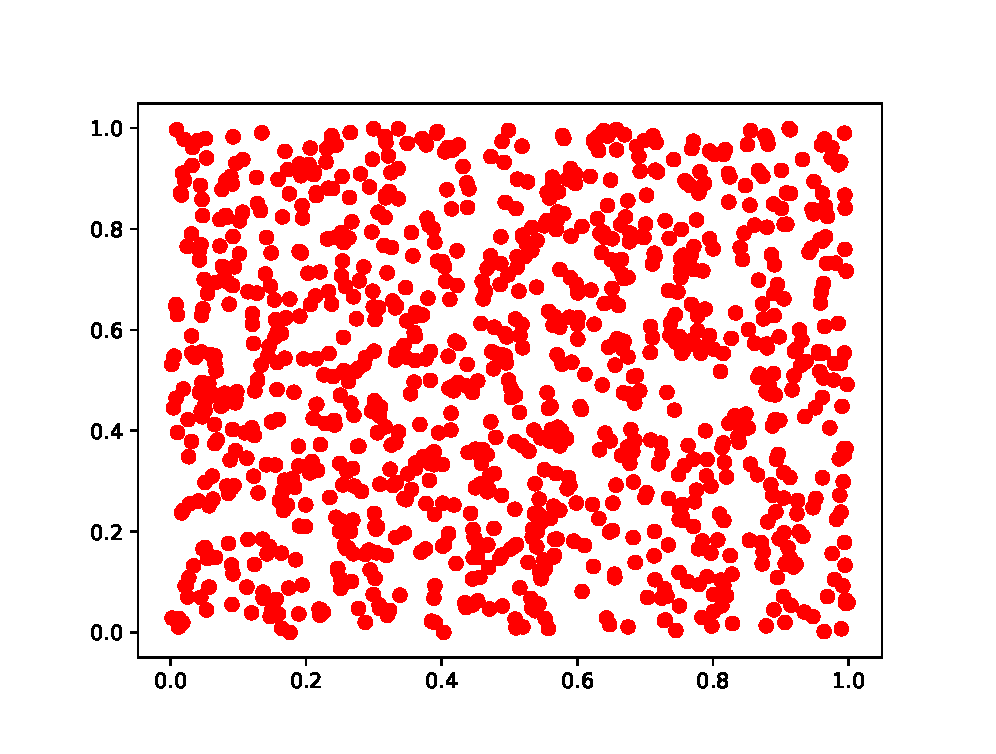
\includegraphics[width=1.2\textwidth]{figures/randu.eps}
        \caption{RANDU}
    \end{minipage}
    \end{figure}
\end{document}

\section*{exercise 2}
\begin{figure}
    \includegraphics{figures/times.png}
\end{figure}
\begin{figure}
    \includegraphics{figures/errors.png}
\end{figure}